\chapter{Implementierung und Evaluation}
\label{ch:Evaluation}

Die folgenden Abschnitte beschreiben jeweils die Implementierung des Prototyps zur Videoaufzeichnung und die Ergebnisse der Evaluation anhand der in \autoref{ch:Bewertungskriterien} aufgeführten Kriterien.
Dabei wird erläutert, wie die einzelnen Komponenten des Prototyps implementiert werden und welche zusätzlichen Komponenten eingesetzt werden müssen, um die geforderte Funktionalität umzusetzen.
Die Frameworks verwenden verschiedene Bezeichnungen für eingebundene Komponenten von Drittanbietern.
Zur einheitlichen Beschreibung werden diese in den folgenden Abschnitten jeweils als Plugins bezeichnet. 

Insgesamt ist festzustellen, dass die Grundfunktionalität der Videoaufzeichnung mit allen untersuchten Frameworks mit vorhandenen Plugins umgesetzt werden kann.
Welche Komponenten verwendet wurden, welche Probleme aufgetreten sind und welche Einstellmöglichkeiten für die Parameter bestehen ist in den Abschnitten \ref{sec:Evaluation_Flutter} bis \ref{sec:Evaluation_ReactNative} beschrieben.
Auch der Zugriff auf den Gerätespeicher zur Speicherung der Videos ist in allen Frameworks möglich.
Dabei ist jedoch aufgefallen, dass kein Framework plattformübergreifende Speicherpfade unterstützt.
Stattdessen muss für jede Plattform ein passender Pfad, angepasst an die jeweilige Dateisystemstruktur, erzeugt werden.
Erste Unterschiede zeigen sich bei der Wiedergabe aufgezeichneter Videos.
Diese ist in Ionic mit Cordova mit allen getesteten Plugins nicht möglich.

\section{Implementierung und Evaluation der Grundfunktionalität}
\subsection{Implementierung mit Flutter}
\label{sec:Evaluation_Flutter}

Für den Zugriff auf Kamerafunktionen steht ein offizielles Dart Package beziehungsweise Plugin zur Verfügung \cite{Dart_Camera}.
Über dieses Plugin ist die Aufzeichnung von Videos unter Android und iOS möglich und einige Parameter können angepasst werden.
Für die Speicherung ist kein zusätzliches Plugin notwendig, der Zugriff auf Gerätespeicher ist in Flutter bereits integriert.
Zur Wiedergabe der Videos wird das offizielle Video-Player-Plugin verwendet \cite{Dart_Video}.

Die erforderlichen Anforderungen, sowie die Wiedergabe von Videos, können somit mit Flutter vollständig umgesetzt werden.
Allerdings gibt es einige Einschränkungen bei den einstellbaren Parametern.
So sind weder Belichtungszeit noch ISO-Wert einstellbar, für die Belichtung kann nur ein bestimmtes Offset für ein allgemein helleres beziehungsweise dunkleres Video gesetzt werden.
Zudem kann die Aktualisierung der automatischen Belichtungssteuerung gestoppt werden, die letzte automatische Einstellung bleibt dabei erhalten.
Der Fokus kann ebenfalls nicht komplett manuell gewählt werden, stattdessen kann ein Punkt auf dem Bildschirm ausgewählt werden, welcher vom Autofokussystem als Ausgangspunkt verwendet wird.
Für das Bildformat stehen bis zu fünf verschiedene Voreinstellungen zur Verfügung, wobei die Verfügbarkeit vom verwendeten Gerät abhängt.
Weißabgleich, Videocodec und Bildrate lassen sich ebenfalls nicht einstellen.
Außerdem konnte nicht jeder verfügbare Sensor des Android-Testsmartphones ausgewählt werden.


\subsection{Implementierung mit Ionic und Cordova}
\label{sec:Evaluation_Ionic}

Allgemein erlaubt Cordova den Zugriff auf native Funktionen, wie die Videoaufzeichnung nur über Plugins.
Erste Quelle für bestehende Plugins ist bei Verwendung von Ionic als UI-Toolkit die Sammlung offiziell unterstützter und getesteter Plugins, die unter \url{https://ionicframework.com/docs/native/} bereitsteht.
Hier konnten drei Plugins identifiziert werden, welche den Zugriff auf Kamerafunktionen ermöglichen.
Das naheliegende Plugin \textit{cordova-plugin-camera} erlaubt nur die Aufzeichnung von Bildern \cite{Cordova_Camera}.
Das Plugin \textit{cordova-plugin-camera-preview} ermöglicht zwar die Aufzeichnung von Videos, jedoch ist diese Funktion nur auf Android-Geräten verfügbar \cite{Cordova_CameraPreview}.
Lediglich das Plugin \textit{cordova-plugin-media-capture} erlaubt die Aufzeichnung von Videos auf allen Plattformen \cite{Cordova_MediaCapture}.
Jedoch verwendet dieses Plugin eine vom Betriebssystem bereitgestellte Aufzeichnungsfunktion, sodass aus der App heraus nur das Videoaufzeichnungsfenster geöffnet werden kann.
Dabei sind keinerlei Einstellungen der in \autoref{tab:parameter_support} aufgeführten Parameter möglich.
Auch außerhalb der offiziellen Sammlung von verifizierten Plugins konnten keine Plugins identifiziert werden, welche die Einstellung einiger Parameter unterstützen.
Die Speicherung aufgezeichneter Videos erfolgt ohne zu erkennende Einschränkungen über das offizielle Plugin \textit{cordova-plugin-file} \cite{Cordova_File}.
Die Wiedergabe der Videos hingegen konnte weder über das HTML-Video Element noch durch ein Plugin realisiert werden. 

Damit sind die erforderlichen Anforderungen zwar umgesetzt, jedoch werden keine der optionalen Anforderungen erfüllt.
Um die optionalen Anforderungen umzusetzen, müssten spezifische Plugins implementiert werden.
Dementsprechend ist die Implementierung einer Videoaufzeichnungsanwendung mit Ionic und Cordova nur stark eingeschränkt möglich.


\subsection{Implementierung mit Xamarin}
\label{sec:Evaluation_Xamarin}

Da Xamarin prinzipiell die Nutzung der nativen \acp{API} unterstützt, sind theoretisch alle Kamerafunktionen nutzbar.
Allerdings sollen im Rahmen dieser Arbeit nur die vorhandenen plattformübergreifenden Abstraktionen des Frameworks genutzt werden.
Die offizielle Bibliothek \textit{Xamarin.Essentials} ermöglicht neben der Nutzung weiterer nativer Funktionen auch den Zugriff auf verschiedene Kamerafunktionen.
Zum Zugriff auf die Kamera steht eine stark vereinfachte \ac{API} über die statische Klasse \textit{MediaPicker} bereit \cite{Xamarin_MediaPicker}.
Wie das, in der Implementierung mit Cordova eingesetzte Plugin, wird auch hier die Aufzeichnung von Videos über die vom Betriebssystem bereitgestellte Aufzeichnungsfunktion realisiert.
Deshalb ist auch hier die Aufzeichnung von Videos zwar möglich, jedoch können keine Parameter aus der Anwendung heraus gesetzt werden.
Der Zugriff auf den Gerätespeicher ist wie bei Flutter ohne zusätzliche Abhängigkeiten möglich.
Die Wiedergabe der Videos ist über ein entsprechendes \ac{UI}-Element der offiziellen Bibliothek \textit{XamarinCommunityToolkit} \cite{Xamarin_CommunityToolkit} ohne Einschränkungen möglich.

Mit Xamarin lassen sich ohne die direkte Verwendung nativer \acp{API} nur die erforderlichen Anforderungen uneingeschränkt erfüllen.
Auch die Wiedergabe der Videos ist ohne Einschränkungen möglich.
Die optionale Einstellbarkeit der Parameter kann hingegen nicht umgesetzt werden.


\subsection{Implementierung mit React Native}
\label{sec:Evaluation_ReactNative}

Für die Videoaufzeichnung mit React Native konnten zwei geeignete Native Modules beziehungsweise Plugins identifiziert werden.
Da das Plugin \textit{react-native-vision-camera} \cite{Vision_Canmera} bei der Einstellung von Parametern mehr Flexibilität bietet als das Pluguin \textit{expo-camera} \cite{Expo_Camera}, wird für die prototypische Implementierung dieses Plugin verwendet.
Für Speicherung und Wiedergabe der Videos müssen zusätzlich \textit{react-native-fs} \cite{ReactNative_FileSystem} respektive \textit{react-native-video} \cite{ReactNative_Video} eingebunden werden.

Die erforderlichen Anforderungen und die Wiedergabe von Videos können mit React Native ohne Einschränkungen umgesetzt werden.
Bei der Einstellbarkeit der Parameter gibt es im Vergleich mit den anderen Frameworks zudem weniger Einschränkungen.
So ist eine freie Wahl des Sensors möglich, auf Basis derer die weiteren Einstellmöglichkeiten abhängig von den Fähigkeiten des Sensors eingeschränkt werden.
Verschiedene Sensoren unterstützen dabei unterschiedliche Kombinationen von Einstellungen, welche als sogenannte Formate abgerufen werden können.
Das Format definiert insbesondere die Auflösung und den Farbraum.
Abhängig vom Format kann die Bildrate für Videoaufnahmen in einem, im Format angegebenen, Bereich eingestellt werden.
Weiterhin kann der Fokus in ähnlicher Art und Weise wie bei Flutter gesetzt werden.
Unter iOS ist zudem die Wahl eines der unterstützten Videocodecs möglich.
Die Belichtungsparameter ISO und Belichtungszeit können jedoch nicht eingestellt werden.


\subsection{Vergleich allgemeiner Kriterien}


\begin{figure}[ht]
  \centering 
  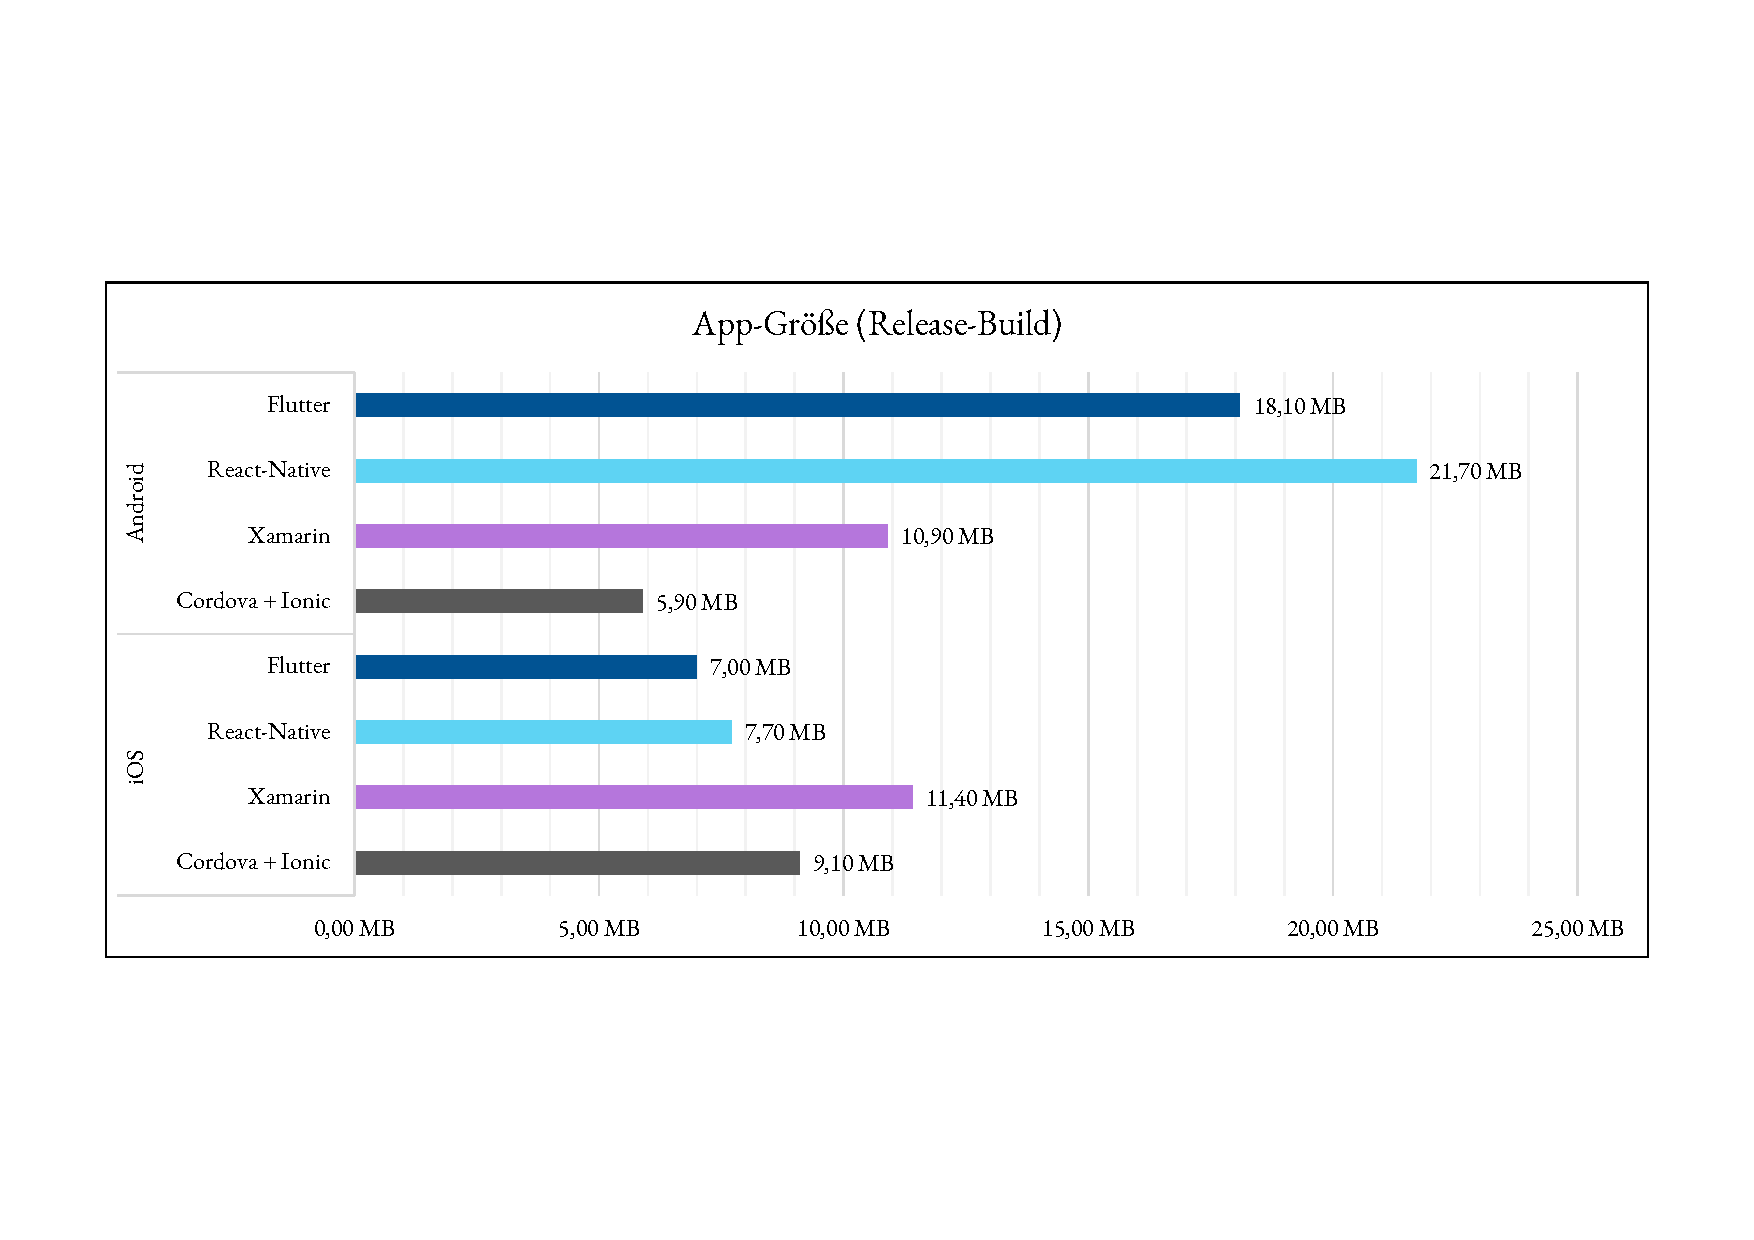
\includegraphics[trim=1.8cm 4.5cm 1.8cm 4.5cm, clip, width=0.9\textwidth]{app_size.pdf}
  \caption{Vergleich der Größe eines Release-Builds abhängig von Framework und Betriebssystem.}
  \label{fig:app_size}
\end{figure}

\begin{figure}[ht]
  \centering 
  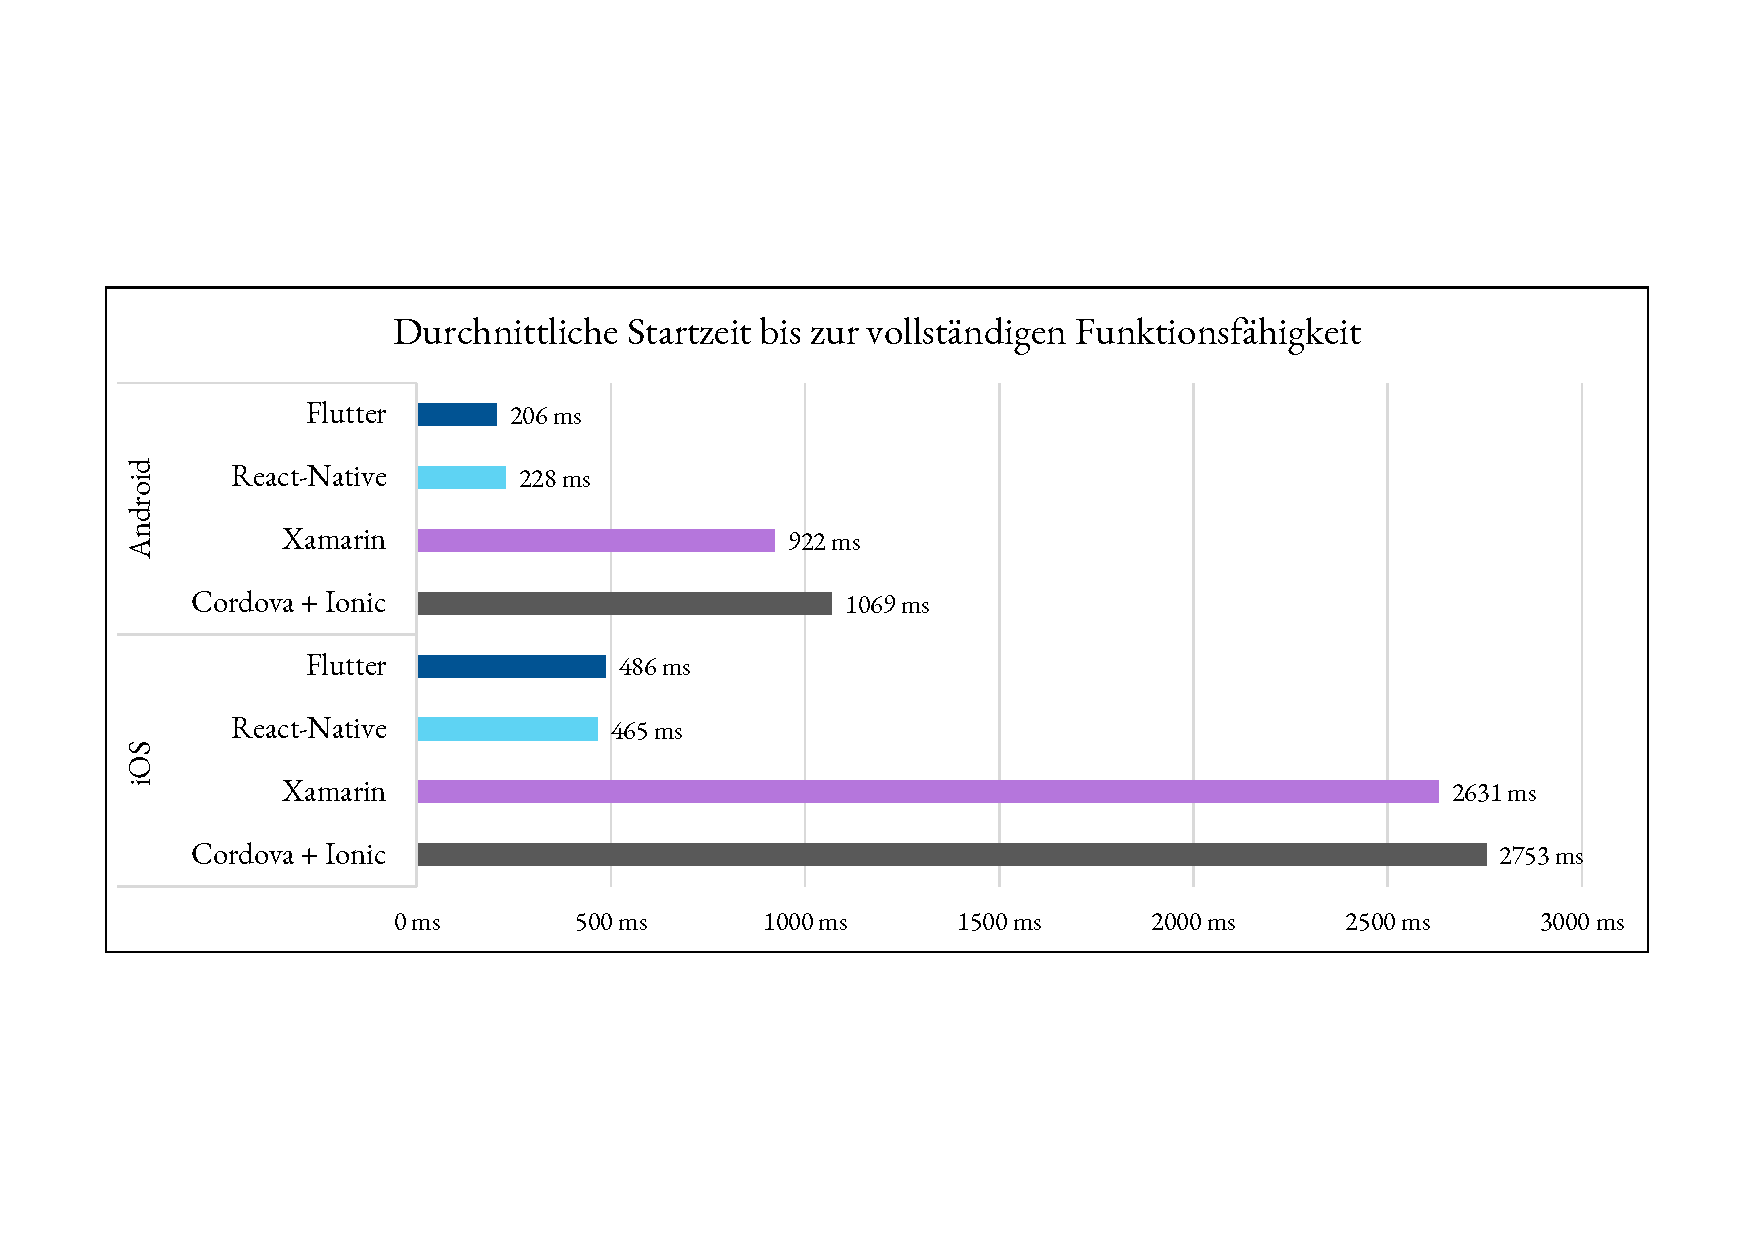
\includegraphics[trim=1.8cm 4.5cm 1.8cm 4.5cm, clip, width=0.9\textwidth]{launch_time.pdf}
  \caption{Vergleich der Zeit bis zur vollständigen Funktionsfähigkeit des Prototyps abhängig von Framework und Betriebssystem.}
  \label{fig:launch_time}
\end{figure}

\begin{figure}[ht]
  \centering 
  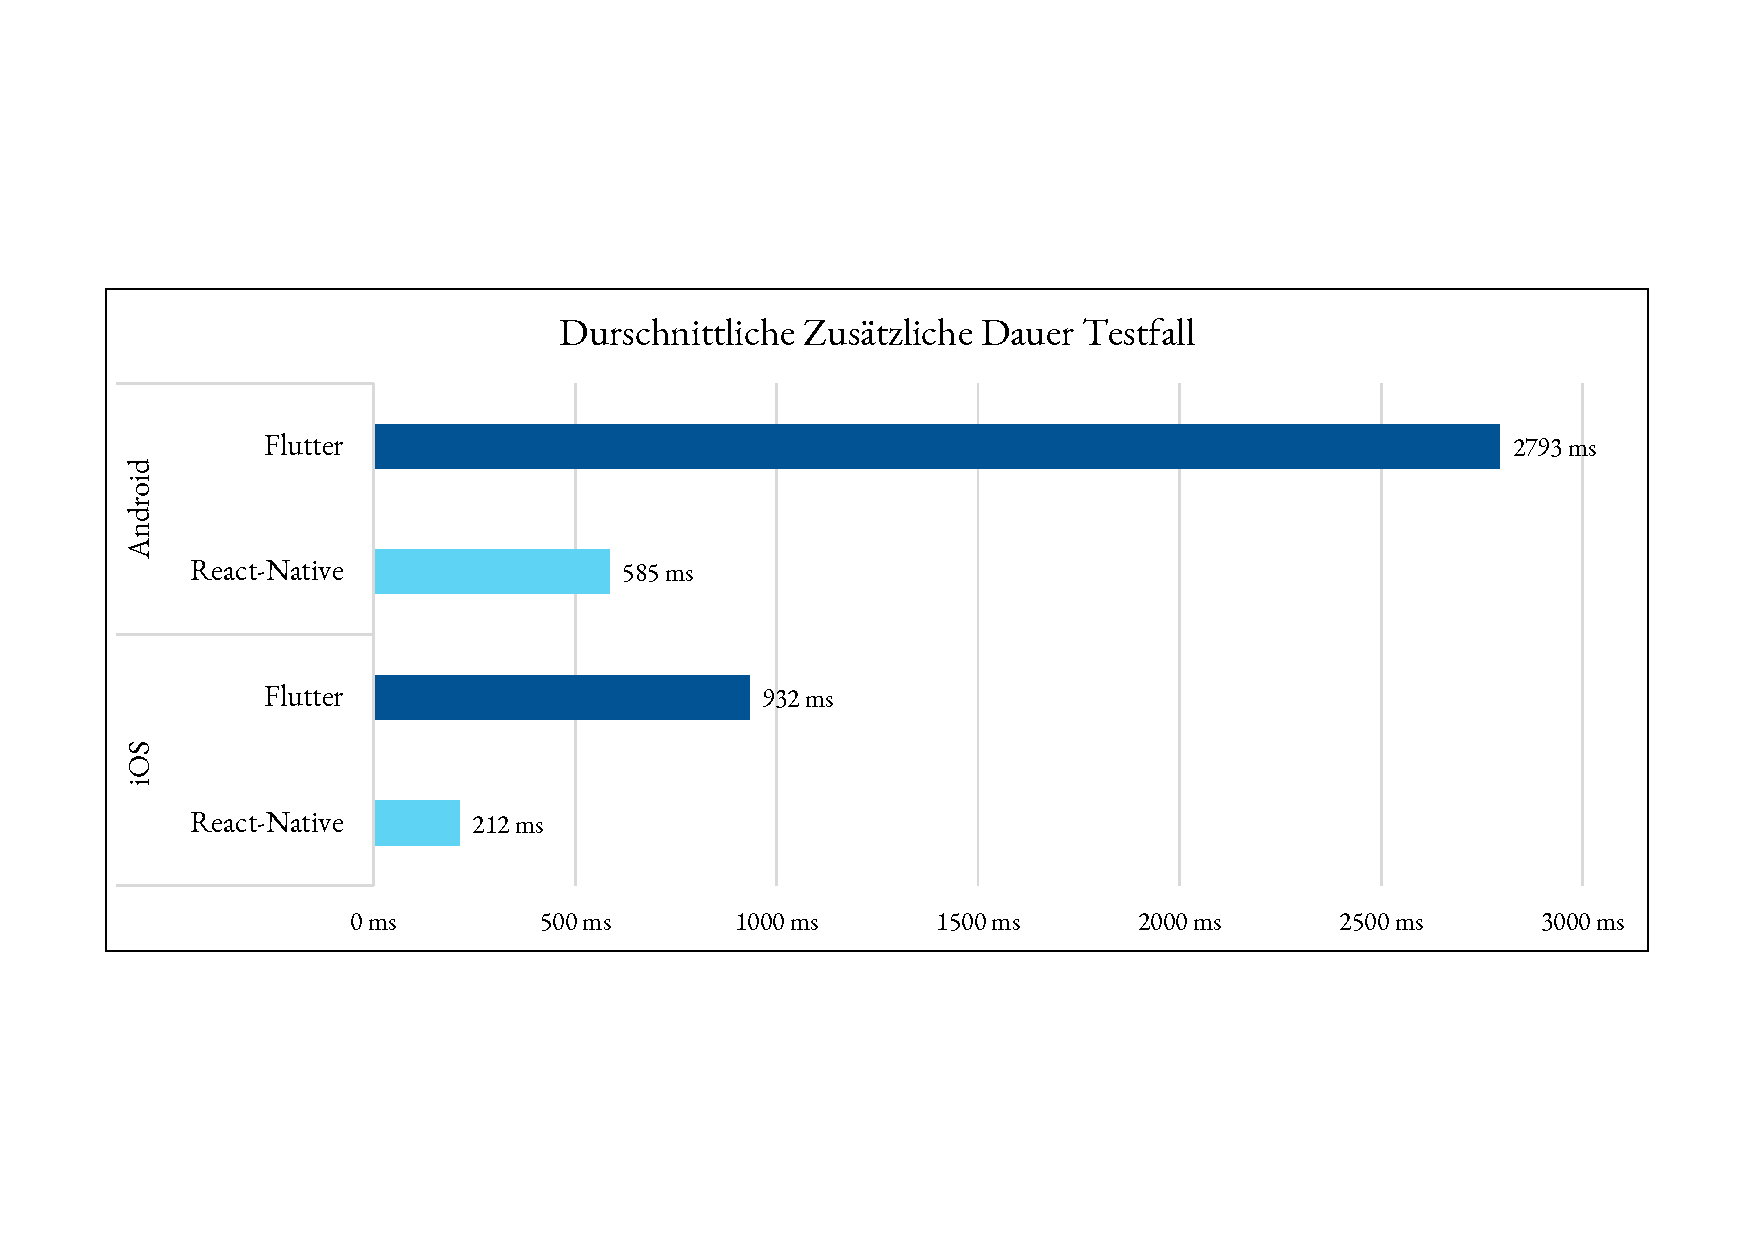
\includegraphics[trim=1.8cm 4.5cm 1.8cm 4.5cm, clip, width=0.9\textwidth]{testcase.pdf}
  \caption{Vergleich der für die Aufzeichnung und Speicherung von zehn Sekunden Video zusätzlich benötigten Zeit abhängig von Framework und Betriebssystem.}
  \label{fig:testcase}
\end{figure}